% Apartado 2.2 - Generacion y caracterizacion de senales (20 puntos) - BLOQUE 1
% Desarrollo completo y cifras en docs/2_2_senales.md
% Codigo: src/senales.py   Pruebas: pruebas/test_senales.py
% Figuras: fig_22_caso_1.png, fig_22_caso_2.png, fig_22_caso_3.png, fig_22_comparacion.png

\section{Generación y caracterización de señales}
\label{sec:senales}

\subsection{Parámetros y casos de prueba}

La frecuencia de muestreo es de 16\,kHz. La componente útil más alta está en
1320\,Hz y la interferencia más alta en 3500\,Hz, de modo que el margen sobre
Nyquist es amplio y ninguna componente se pliega.

La duración es de 2,048\,s, que a 16\,kHz son exactamente 32\,768 muestras. El
valor no es arbitrario: es una potencia de dos y un múltiplo entero del bloque
de 1024 muestras, así que el procesamiento por bloques del apartado
\ref{sec:espectral} divide la señal en 32 bloques exactos sin rellenar el
último con ceros, y la FFT radix-2 propia puede analizar la señal completa de
una sola vez. Con $N=1024$ la resolución por bloque es
$\Delta f = f_s/N = 15{,}6$\,Hz y la latencia $N/f_s = 64$\,ms.

Los tres casos comparten la misma señal útil, un multitono de 440, 880 y
1320\,Hz con amplitudes relativas 1{,}00, 0{,}55 y 0{,}30 y fases de
$0^\circ$, $35^\circ$ y $-50^\circ$. Compartirla es deliberado: cualquier
diferencia que se mida después se le puede atribuir al ruido y no a la señal.

\begin{table}[H]
\centering\small
\caption{Los tres casos de prueba. Cada uno usa su propia semilla.}
\begin{tabular}{llrl}
\toprule
Caso & Ruido & SNR objetivo & Qué pone a prueba \\
\midrule
\texttt{caso\_1} & tonal en 3500\,Hz        & 2,0 dB & interferencia separada de la banda útil \\
\texttt{caso\_2} & blanco                   & 0,0 dB & ruido repartido por todo el espectro \\
\texttt{caso\_3} & banda 800--1500\,Hz      & 3,0 dB & el ruido se solapa con la banda útil \\
\bottomrule
\end{tabular}
\end{table}

El ruido de banda del tercer caso no se genera con un filtro de biblioteca sino
enmascarando el espectro de ruido blanco con un paso banda de bordes de coseno
elevado y 50\,Hz de transición. Es equivalente para el propósito y deja la
generación sin más dependencias que \texttt{numpy}.

\subsection{Verificación de la SNR}

La amplitud del ruido se escala por cálculo directo,
\begin{equation}
\alpha=\sqrt{\frac{\sum_n s^2[n]}{\sum_n r^2[n]\cdot 10^{\,\mathrm{SNR}/10}}},
\end{equation}
de modo que la relación señal a ruido sale exacta por construcción. Las tres
señales se normalizan después con una \emph{misma} ganancia, y por ser común no
altera la relación entre ellas.

\begin{table}[H]
\centering\small
\caption{La SNR coincide con la configurada. La única diferencia es la
cuantización a 16 bits del archivo WAV.}
\begin{tabular}{lrrrr}
\toprule
Caso & Objetivo & Punto flotante & Leída del WAV & Diferencia \\
\midrule
\texttt{caso\_1} & 2,0 dB & 2,0000 dB & 1,9999 dB  & $-0{,}0001$ dB \\
\texttt{caso\_2} & 0,0 dB & 0,0000 dB & $-0{,}0003$ dB & $-0{,}0003$ dB \\
\texttt{caso\_3} & 3,0 dB & 3,0000 dB & 2,9998 dB  & $-0{,}0002$ dB \\
\bottomrule
\end{tabular}
\end{table}

\subsection{Caracterización temporal y espectral}

\begin{figure}[H]
\centering
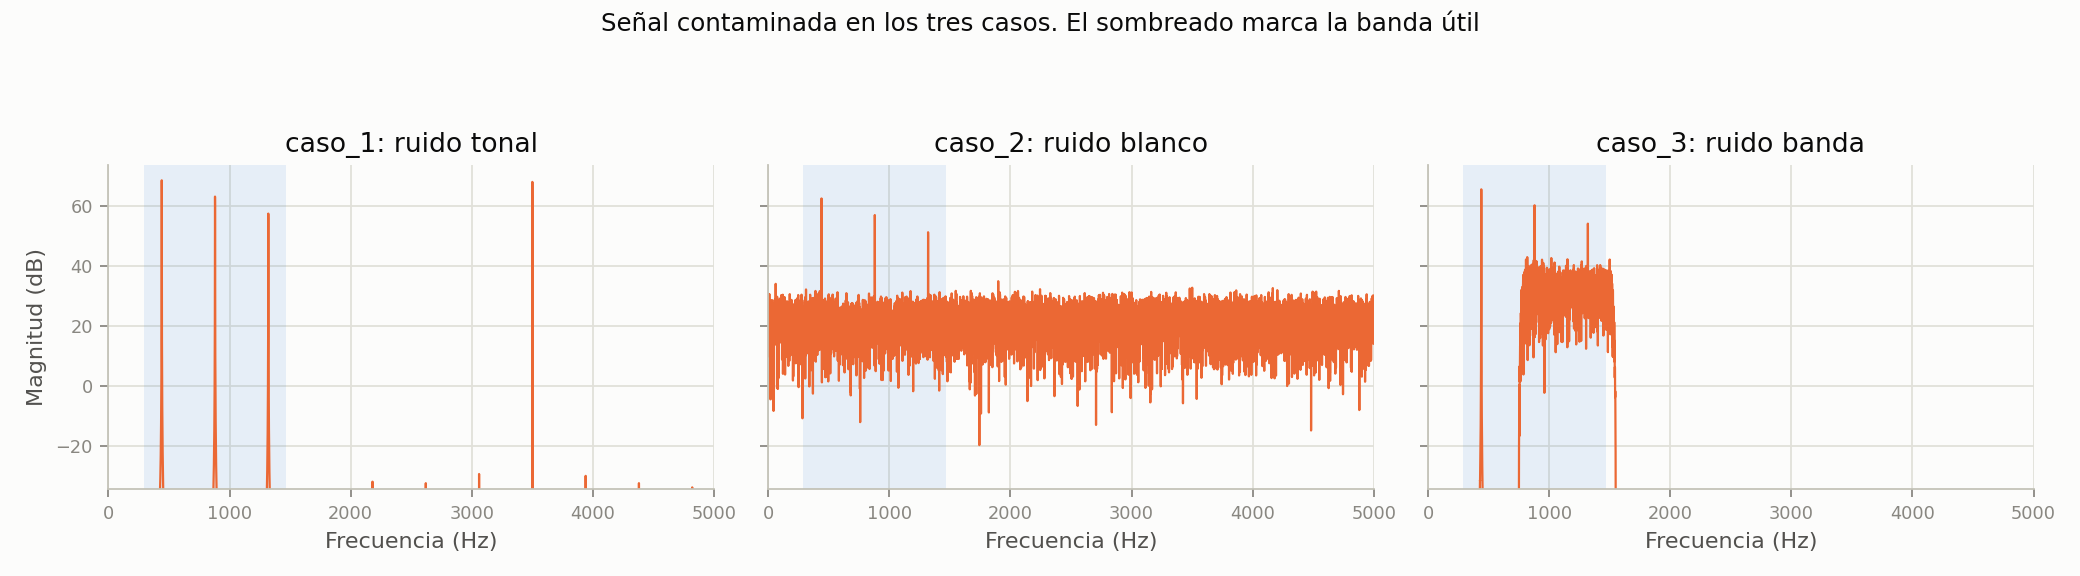
\includegraphics[width=\textwidth]{fig_22_comparacion.png}
\caption{Señal contaminada en los tres casos. El sombreado marca la banda útil.
Se ve de un vistazo por qué el tercer caso es el difícil: su ruido cae encima de
dos de los tres tonos.}
\label{fig:comparacion}
\end{figure}

Las figuras \texttt{fig\_22\_caso\_1}, \texttt{fig\_22\_caso\_2} y
\texttt{fig\_22\_caso\_3} traen, para cada caso, la señal en el tiempo, el
espectro de magnitud, la fase y la distribución de energía por bandas.

\begin{table}[H]
\centering\small
\caption{Energía de la señal contaminada repartida por bandas, en porcentaje.
Las tres firmas son distintas y se leen directo de la tabla.}
\begin{tabular}{lrrrrrr}
\toprule
Banda (Hz) & 0--250 & 250--500 & 500--1000 & 1000--2000 & 2000--4000 & 4000--8000 \\
\midrule
\texttt{caso\_1} & 0,0 & 44,0 & 13,3 & 4,0 & \textbf{38,7} & 0,0 \\
\texttt{caso\_2} & 1,5 & 37,7 & 13,5 & 9,5 & 12,9 & \textbf{25,0} \\
\texttt{caso\_3} & 0,0 & 47,9 & 24,7 & \textbf{27,3} & 0,0 & 0,0 \\
\bottomrule
\end{tabular}
\end{table}

La fase lo muestra todavía más claro que la magnitud. En el primer caso la fase
de los tres tonos útiles se conserva intacta y solo aparece una componente nueva
en 3500\,Hz. En el tercero la fase es azar en toda la banda 800--1500\,Hz: ahí la
información original ya se perdió.

\subsection{Identificación automática del ruido}

El nodo de adquisición del proyecto tiene que decidir solo qué clase de ruido
está viendo. Se proponen tres características, medidas sobre los propios casos.

La \textbf{planitud espectral} --- media geométrica entre media aritmética de la
densidad de potencia --- vale 1 para ruido blanco perfecto y tiende a cero cuando
la energía se concentra en pocos bines.

\begin{table}[H]
\centering\small
\caption{Planitud espectral. Separa los tres casos por varios órdenes de magnitud.}
\begin{tabular}{lrrr}
\toprule
 & Señal limpia & Ruido solo & Señal contaminada \\
\midrule
\texttt{caso\_1} & $2{,}7\cdot10^{-15}$ & $1{,}2\cdot10^{-19}$ & $1{,}9\cdot10^{-14}$ \\
\texttt{caso\_2} & $8{,}3\cdot10^{-15}$ & $\mathbf{0{,}556}$   & $\mathbf{0{,}277}$ \\
\texttt{caso\_3} & $4{,}4\cdot10^{-15}$ & $3{,}2\cdot10^{-8}$  & $1{,}1\cdot10^{-8}$ \\
\bottomrule
\end{tabular}
\end{table}

La \textbf{razón entre el pico del espectro y su mediana} vale 181\,dB en el
primer caso, 41\,dB en el segundo y 124\,dB en el tercero: cuando hay una
interferencia tonal, un solo bin se dispara muy por encima de la mediana,
mientras que con ruido blanco no hay ningún bin dominante.

La \textbf{longitud del tramo contiguo por encima de la mediana} distingue los
dos casos que tienen planitud baja: una interferencia tonal ocupa uno o dos
bines, un ruido de banda ocupa un tramo largo.

Con esas tres medidas el nodo espectral puede escoger su estrategia sin
intervención: atenuación proporcional al piso de ruido si la planitud es alta,
rechazo estrecho centrado en el bin detectado si hay un pico dominante, y
rechazo de banda con el ancho medido si hay un tramo contiguo.

\subsection{Qué información no se puede recuperar}
\label{sec:limite}

La respuesta se ve midiendo la SNR \emph{tono por tono}, es decir cuánta energía
de ruido cae encima de cada componente útil.

\begin{table}[H]
\centering\small
\caption{SNR medida en una ventana de $\pm 60$\,Hz alrededor de cada tono útil.
«Limpio» significa que lo único medible en esa banda es la fuga de la ventana de
análisis, más de 100\,dB por debajo.}
\begin{tabular}{lccc}
\toprule
Tono útil & \texttt{caso\_1} & \texttt{caso\_2} & \texttt{caso\_3} \\
\midrule
440\,Hz  & limpio & 16,9 dB & limpio \\
880\,Hz  & limpio & 12,1 dB & \textbf{4,2 dB} \\
1320\,Hz & limpio & 6,1 dB  & $\mathbf{-0{,}9}$ \textbf{dB} \\
\bottomrule
\end{tabular}
\end{table}

En el primer caso ningún tono útil comparte frecuencia con el ruido, así que un
filtro puede quitar la interferencia entera sin tocar la señal y la información
se recupera completa. En el tercero el tono de 1320\,Hz tiene \emph{menos
energía que el ruido que lo acompaña}. Ahí no hay filtro lineal e invariante en
el tiempo que sirva: la operación que separaría señal de ruido tendría que
distinguir dos contribuciones que ocupan el mismo bin de la DFT, y la DFT no
guarda ninguna otra información con la cual distinguirlas.

Lo que sí sobrevive cuando señal y ruido comparten frecuencia es la energía
total de la banda, pero no el reparto entre una y otra: en el tercer caso la
banda de 1320\,Hz tiene 2,15 veces la energía que tenía en la señal limpia, y
todo ese exceso es ruido. La fase solo se conserva donde la señal todavía domina.

La consecuencia práctica para el apartado \ref{sec:espectral} es que cualquier
método que atenúe la banda 800--1500\,Hz en el tercer caso va a degradar los
tonos de 880 y 1320\,Hz. No es un defecto del método sino el límite del
problema, y lo único que queda por decidir es cuánto se sacrifica de cada lado.
